\chapter{考察}
\section{3次の基底関数を用いたIGA解析}
\subsection{内圧を受ける厚肉円筒の解析}

図~\ref{fig:iga ER 01},図~\ref{fig:iga ER 02}における
2次の基底関数を用いた場合と3次の基底関数を用いた場合の
それぞれの近似直線の収束率を表~\ref{table:Convergence rate}に示す.

\begin{table}[hbtp]
  \caption{Convergence rate}
  \label{table:Convergence rate}
  \centering
  \scalebox{1.0}{
    \begin{tabular}{|c|c|c|}
      \hline
      Order of basis function & 2 & 3 \\
      \hline
      Convergence rate of $\sigma_{rr}$ & 1.1598 & 1.1609 \\
      \hline
      Convergence rate of $\sigma_{\theta\theta}$ & 1.9100 & 1.9146 \\
      \hline
    \end{tabular}
  }
\end{table}

\noindent
この結果から,同自由度数の解析においては全ての解析で
3次の基底関数を用いた場合の方が2次の基底関数を用いた場合より,
誤差ノルムが小さくなっていることがわかる.
収束率の数値からも,IGA解析では3次の基底関数を用いた方が
より少ない自由度で同程度の精度の解析結果が得られることが確認された.

\section{3次の基底関数を用いた重合パッチ法解析}
\subsection{遠方で一様引張を受ける円孔を有する平板の解析}
\subsubsection{各パッチでの基底関数の次数の組み合わせによる解析精度検証}
グローバルパッチとローカルパッチの基底関数の次数を,
(a)(2次,2次),
(b)(2次,3次),
(c)(3次,2次),
(d)(3次,3次)としてグローバルパッチの分割数を固定してローカルパッチの分割数を変更することで
各パッチでの基底関数の次数の組み合わせによる誤差の影響を比較した.

図~\ref{fig:ERNr},図~\ref{fig:ERNt}に示す誤差ノルムの結果からは,
同自由度における全ての解析で(d)が最も精度が高く,(c)が最も精度が低い結果となった.
(a)と比較して(b)はやや精度が高くなったがほとんど変わりはなく,
(d)は大きく精度が向上した.

図~\ref{fig:contour22}~図~\ref{fig:contour33}に示す
$y$方向応力$\sigma_{yy}$の応力分布図の比較では,
(a)と(b)には各所で解が振動するような現象が確認されるが,
(d)は滑らかな分布となった.
また,(c)は理論解から大きく外れた分布となっており,
誤差ノルムの結果からも精度が大きく低下する組み合わせであると考えられる.
グローバルパッチとローカルパッチの次数の組み合わせを決定する際には,
(d)を採用すると最も精度が高くなると考えられる.

\newpage

\subsubsection{グローバルパッチの分割数を固定してローカルパッチの分割数を変更した解析}
グローバルパッチの分割数を固定してローカルパッチの分割数を変更することで,
ローカルパッチの分割数による誤差の影響を2次と3次の基底関数を用いた場合で比較した.

円孔縁の主応力$\sigma_1,\sigma_2$の分布及び
$x$軸上の$y$方向応力$\sigma_{yy}$の分布の結果からは,
全ての解析で3次の基底関数を用いた解析の方が2次の基底関数を用いた解析より
精度が向上し,滑らかな分布となることが確認された.
また2次と3次の基底関数の場合で共に,ローカルパッチの分割数が比較的少ない場合でも
理論解とよく合っており,さらにローカルパッチの分割数を細かくするとローカルパッチ内部での
分布がよりよくなると考えられる.

$y$方向応力$\sigma_{yy}$の応力分布図の比較では,3次の基底関数を用いた方が
滑らかな分布を示し,2次の基底関数を用いた場合に見られる振動するような
解の分布が一切見られなかった.

\subsubsection{ローカルパッチの分割数を固定してグローバルパッチの分割数を変更した解析}
ローカルパッチの分割数を固定してグローバルパッチの分割数を変更することで,
グローバルパッチの分割数による誤差の影響を2次と3次の基底関数を用いた場合で比較した.

円孔縁の主応力$\sigma_1,\sigma_2$の分布及び
$x$軸上の$y$方向応力$\sigma_{yy}$の分布の結果からは,
2次と3次の基底関数を用いた場合の精度はほとんど変わらず,同じような分布を示した.
グローバルパッチの分割数が粗い場合には2次と3次の基底関数を用いた場合でいずれも
精度の上限が見られ,理論解から大きく外れる結果が得られた.
ローカルパッチを十分に細かくして解析を行っているため,
これ以上ローカルパッチの分割数を細かくしても
精度は向上せず,
ローカルパッチ内部の分布がより滑らかになるだけで,
解の誤差はほぼ収束していると考えられる.
この結果からローカルパッチの分割数に起因する誤差より
グローバルパッチの分割数,要素サイズに起因する誤差の方が大きいと考えられる.
ローカルパッチ内部の分布に関しては,
2次より3次の基底関数を用いた方が小さな振動がなくなり
滑らかな分布となった.

$y$方向応力$\sigma_{yy}$の応力分布図の比較では,
3次の基底関数を用いた解析の方が2次の基底関数を用いた解析より
滑らかな分布となった.

\subsubsection{グローバルパッチの分割数を固定してローカルパッチのサイズと分割数を変更した解析}
グローバルパッチの分割数を固定してローカルパッチのサイズと分割数を変更し,
誤差ノルムを用いて誤差の大きさを定量的に示すことで,
重合パッチ法解析における2次と3次の基底関数を用いた場合の誤差精度,
グローバルパッチの要素サイズとローカルパッチの全体サイズの比と誤差ノルムの関係を検証した.

各ローカルパッチサイズでの半径方向応力$\sigma_{rr}$の分布の結果からは,
同自由度の解析では全ての解析で,2次の基底関数を用いた場合より3次の基底関数を用いた場合の方が
誤差ノルムが小さくなったため,
グローバルパッチの分割数を固定してローカルパッチの分割数を変更した解析と
ローカルパッチの分割数を固定してグローバルパッチの分割数を変更した解析と
併せて考えると,
重合パッチ法解析においてもIGA解析と同様に
3次の基底関数を用いた場合の方が2次の基底関数を用いた場合より高精度となると
考えられる.

\newpage

また,各ローカルパッチサイズの全体の代表長さを$(r_2 - r_1)\ $mm,
グローバルパッチの要素の代表長さを要素の1辺の長さ$d$mmとし,
その比$(r_2 - r_1)/d$と,
各サイズの解析において自由度数が最も大きい
グローバルパッチの分割数$30\times30$,ローカルパッチの分割数$30\times30$の場合での
半径方向応力$\sigma_{rr}$,
周方向応力$\sigma_{\theta\theta}$の誤差ノルムの関係を図~\ref{fig:s-iga04 r},
図~\ref{fig:s-iga04 theta}に示す.

\begin{figure}[hbtp]
  \begin{tabular}{cc}
    \begin{minipage}[t]{0.45\hsize}
      \centering
      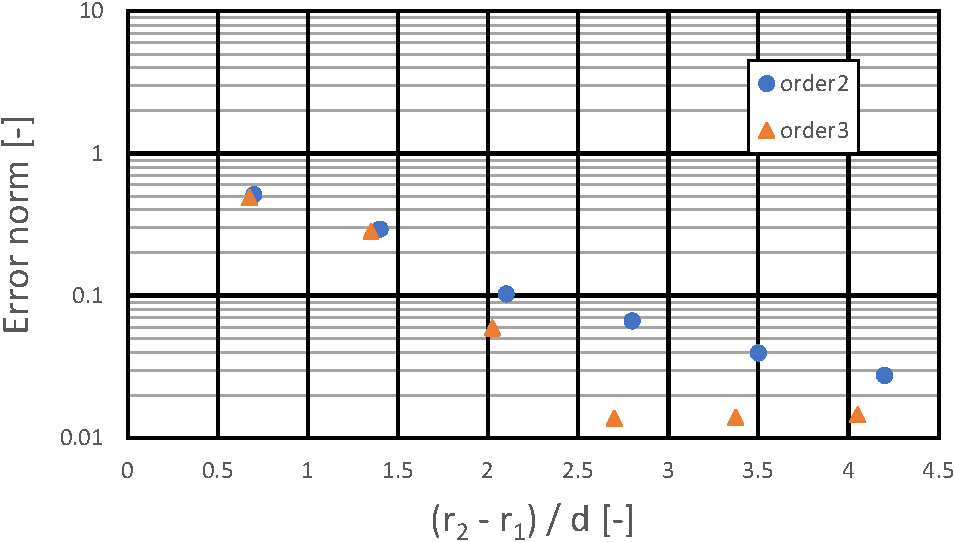
\includegraphics[keepaspectratio, scale=0.4]
      {fig/result_data_etc/s-iga04/r-crop.pdf}
      \caption{Relationship between ratio of Local patch size to Global element size and Error norm of $\sigma_{rr}$}
      \label{fig:s-iga04 r}
    \end{minipage} &
    \begin{minipage}[t]{0.45\hsize}
      \centering
      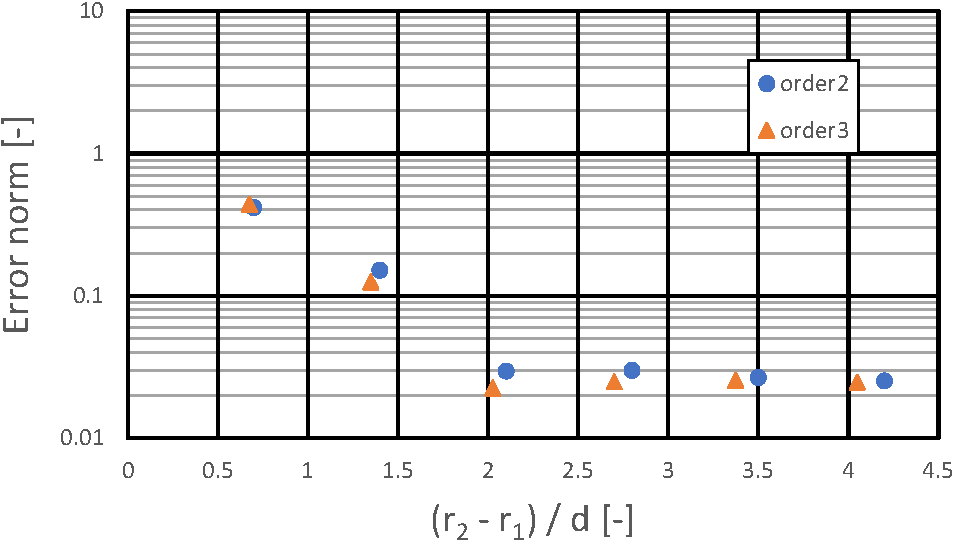
\includegraphics[keepaspectratio, scale=0.4]
      {fig/result_data_etc/s-iga04/theta-crop.pdf}
      \caption{Relationship between ratio of Local patch size to Global element size and Error norm of $\sigma_{\theta\theta}$}
      \label{fig:s-iga04 theta}
    \end{minipage}
  \end{tabular}
\end{figure}

\noindent
この結果からグローバル要素に対するローカルパッチサイズの比が2倍に満たないときは
解析精度がかなり悪くなっており,同自由度ではローカルパッチサイズの比が約2.5倍以上のときに
最も精度が高くなることが確認された.
ただし,この比が約4.5倍を超えたあたりから本研究の連立一次方程式の解法であるCG法が
収束しなくなり安定した解が得られなくなったため,
2次と3次の基底関数のいずれの場合においても,
このサイズ比を約2.5倍から4倍の間に設定すると著しく解析精度が落ちる現象を防ぐことができ,
より精度の高い解が得られると考えられる.
